\documentclass{article}

% Required for inserting images
\usepackage{graphicx}


% to have more colors avelable
\usepackage{xcolor}

% to insert hiperlinks
\usepackage[colorlinks=true,linkcolor=cyan]{hyperref}

% to have better references
\usepackage[noabbrev]{cleveref}

% to use prefix for references
\usepackage{etoolbox}

% rule for reference to fugures
\pretocmd{\thefigure}{F}{}{}


\title{Use Of Jigsaw Puzzle Solving Algorithms In The Real World}
\author{Luca Sartore}
\date{May 2023}

\begin{document}

\maketitle

\newpage

% make the table of content without the hiperlink color
{
  \hypersetup{linkcolor=black}
  \tableofcontents
}

\newpage

\section{Abstract}
The jigsaw puzzle problem has been in the eye of computer scientists for a while,
and some clever solutions have already been found. These algorithms are made to
work with a “digital” jigsaw puzzle [\ref{fig:figure_digital_puzzle}],
there aren't papers (at least not popular enough to be searchable)
that try to apply the solution
to a “real world” jigsaw puzzle [\ref{fig:figure_real_puzzle}].\newline
The problem has been tackled by some small projects. But, as said earlier,
the process and eventual challenges has never been documented by a paper,
this wants to be the first.\newline
As a Bonus the paper will also cover the creation of a user friendly app
that will be open source and free to use.

\section{Introduction}
\subsection{Classification}
This paper will focus on type 2 puzzles. A type 2 puzzle is a puzzle where the position, and the orientation of each piece is unknown. 
\subsection{Digital vs Real-World Jigsaw Puzzles}

There is  another important distinction between different types of puzzles. They can be divided into “digital” and “real world” jigsaw puzzles.


% figure of digital jigsaw puzzle    
\begin{figure}[h]
    \caption{An example of a “digital” jigsaw  puzzle}\label{fig:figure_digital_puzzle}
    \centering
    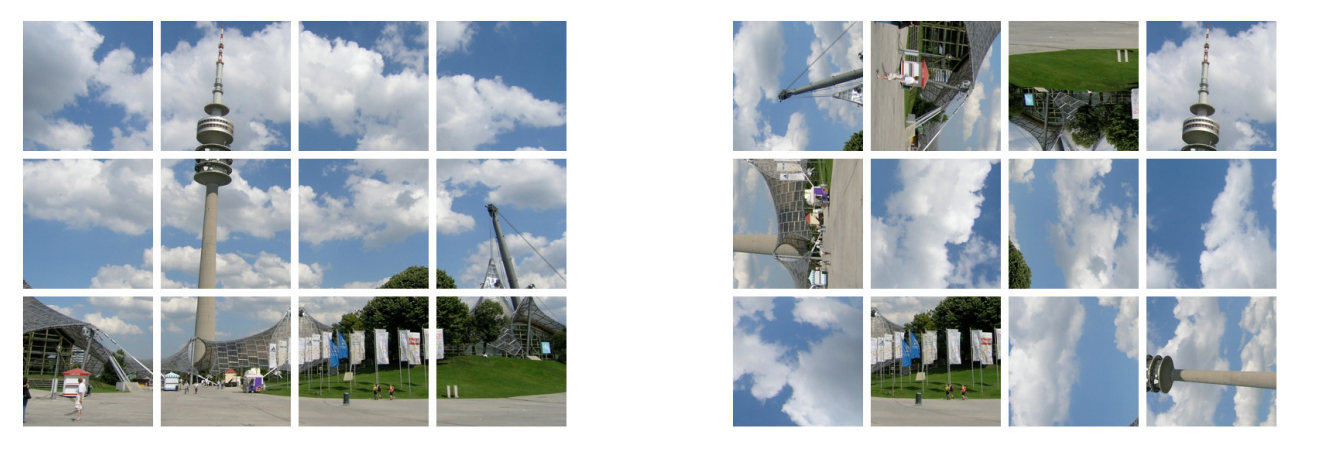
\includegraphics[height=0.25\textwidth]{pictures/digital_puzzle.png}
\end{figure}

% figure of real jigsaw puzzle    
\begin{figure}[h]
    \caption{An example of a “real world” jigsaw  puzzle}\label{fig:figure_real_puzzle}
    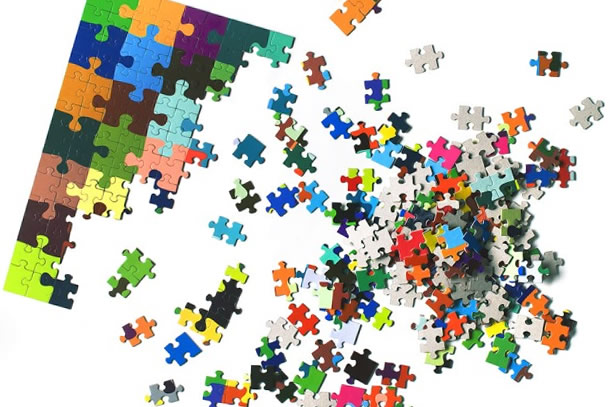
\includegraphics[height=0.25\textwidth]{pictures/real_puzzle.jpg}
    \centering

\end{figure}

The reason this distinction is important is because,
despite the generic concept of the puzzle not changing,
obtaining accurate matches of a piece's characteristics
is far easier with a digital puzzle,
since there are far less things that can go wrong.


% figure of a mesurement error
\begin{figure}[h]
    \caption{An example of what can go wrong when dealing with the real world}\label{fig:figure_measurement_error}
    
\includegraphics[height=0.25\textwidth]{pictures/example_bad_piece.jpg}
    \centering

\end{figure}

\section{Previous Literature}
This section will analyze 3 different algorithms that have been proposed
as a solution of type 2 puzzles. The objective is to understand the
strengths and the weaknesses of each one, to build up some knowledge
that will be useful for the next section.

\subsection{General Structure Of The Algorithms}

All the algorithms that will be analyzed are composed of 3 sub algorithms.

\end{document}

